\subsection{Wirelessmodul}
\label{subsec:Wirelessmodul}

Über einen Web-Host soll der User die Möglickeit haben, Getränke auszuwähen und seinem RFID-Chip zuzuordnen, sowie diverse kleinere Einstellungen an der Maschine vorzunemen. Dazu wird ein WiFi-Modul benötigt, welches auch den Webhost bereitstellen kann.

Aufgrund schon bestehender Erfahrungen wurde ein Espressif ESP-Modul ausgewählt. Grundsätzlich standen zwei Modelle zur Auswahl. Das ESP8266 und das ESP32. Für die Cocktailmaschine wurde das ESP32 ausgewählt, da dies Leistungsstärker ist. Die genauen Datenvergleiche sind in Tabelle \ref{tab:ESP} ersichtlich. Das ESP32 unterstützt das Protokoll nach ISO 802.11 b/g/n und kann somit auf 2.4GHz sowie 5GHz arbeiten. Mit dem n-Protokoll und einer Antenne kann so bis zu 150MBit übertragen werden bei einer Bandbreite von 20MHz.


\begin{table}[!h]
\center
\begin{tabular}{|l|c|c|}
\hline
\textbf{MCU}                    & \textbf{Xtensa Single-Core} & \textbf{Xtensa Dual-Core} \\

			                   & \textbf{32-bit L106 (ESP8266)} & \textbf{32-bit LX6 (ESP32)} \\ \hline

802.11 b/g/n     		& HT20                           & HT40                                       \\
Bluetooth              	& No                             & Bluetooth 4.2 and BLE                      \\
Arbeitsfrequenz			& 80 MHz                         & 160 MHz                                    \\
SRAM                   	& No                             & Yes                                         \\
Flash                  	& No                             & Yes                                          \\
GPIO                   	& 17                             & 36                                         \\
SPI/I2C/I2S/UART       	& 2/1/2/2                        & 4/2/2/2                                    \\
ADC                    	& 10-bit                         & 12-bit                                     \\
Ethernet Interface 		& No                             & Yes                                          \\
Touchsensor           	& No                             & Yes                                          \\
Temperatursensor     	& No                             & Yes                                          \\
Hall-Sensor     			& No                             & Yes \\
Arbeitstemperatur    	& -40ºC to 125ºC                 & -40ºC to 125ºC                             \\
Price                  	& \$ (3\$ - \$6)                 & \$\$ (\$6 - \$12)    \\                         
\hline
\end{tabular}
\caption{Vergleich ESP8266 zu ESP32.}
\label{tab:ESP}
\end{table}

Wichtig ist, dass ein ESP ausgewählt wird, welches einen Anschluss für eine abgesetzte Antenne hat, da die Leiterplatte, worauf das Modul verbaut wird, im Gehäuse platziert wird. Dazu eignet sich der Espressif ESP32-32U.

\newpage

In Tabelle \ref{tab:Strapping_pins} sind die Strapping-Pins aufgelistet, welche während dem Startvorgang einen Einfluss auf die Konfiguration des ESP32 haben. Mit diesen Pins kann die Ausgangsspannung des internen Spannungsregler für VDD\_SDIO, der Bootmodus, der Debug-Log-Print während dem Booten sowie das SPI-Timing der Kommunikation mit der SDIO-Schnittstelle des ESP32 konfiguriert werden.

\begin{table}[h!]
\center
\begin{tabular}{|c|c|c|c|c|c|c|}
\hline
\multicolumn{7}{|c|}{\textbf{Ausgangsspannung internen Spannungsregler (VDD\_SDIO)}}\\
\hline
RS232 & ESP & default & \multicolumn{2}{|c|}{\textbf{3.3V}} & \multicolumn{2}{|c|}{\textbf{1.8V}}\\
\hline
\sout{RTS} & \sout{IO12} & Pull-down & \multicolumn{2}{|c|}{\sout{\textcolor{red}{0}}\footnotemark} & \multicolumn{2}{|c|}{\sout{1}}\\
\hline
\multicolumn{7}{|c|}{\textbf{Boot-Modus}}\\
\hline
RS232 & ESP & default & \multicolumn{2}{|c|}{\textbf{SPI-flash Boot}} & \multicolumn{2}{|c|}{\textbf{Download Boot}}\\
\hline
DTR & IO0 & Pull-up & \multicolumn{2}{|c|}{1} & \multicolumn{2}{|c|}{0}\\
\hline
- & IO2 & Pull-down & \multicolumn{2}{|c|}{Egal} & \multicolumn{2}{|c|}{0}\\
\hline
\multicolumn{7}{|c|}{\textbf{Debugging Log Print über U0TXD während Booten}}\\
\hline
RS232 & ESP & default & \multicolumn{2}{|c|}{\textbf{U0TXD Active}} & \multicolumn{2}{|c|}{\textbf{U0TXD Silent}}\\
\hline
RTS & IO12 & Pull-down & \multicolumn{2}{|c|}{\textcolor{red}{1}} & \multicolumn{2}{|c|}{0}\\
\hline
\multicolumn{7}{|c|}{\textbf{Timing\footnotemark des SDIO}}\\
\hline
RS232 & ESP & default & \shortstack{FF Sampling \\ FF Output} & \shortstack{FF Sampling \\ SF Output} & \shortstack{SF Sampling \\ FF Output} & \shortstack{SF Sampling \\ SF Output} \\
\hline
CTS & IO15 & Pull-up & 0 & 0 & 1 & 1 \\
\hline
- & GPIO5 & Pull-up & 0 & 1 & 0 & 1 \\
\hline
\end{tabular}

\caption{Tabelle Pinkonfiguration für Strapping-Pins.}
\label{tab:Strapping_pins}
\end{table}
\footnotetext[6]{Da das ESP32-WROOM-32U einen 3.3V SPI flash integriert hat, kann der MTDI nicht auf 1 gesetzt werden, wenn die Module aufgestartet sind.}
\footnotetext{FF = Fallende Flanke, SF = Steigende Flanke}


\textbf{Spannung des internen Spannungsgeglers (VDD\_SDIO)}

Das ESP32 hat einen eingebauten host controller für SD/SDIO/MMC-Speichergeräte. Dieser kann mit 3.3V (IO12 = 0) oder 1.8V (IO12 = 1) betrieben werden. Wird der Pin auf 1 gesetzt, könnte ein Brown-out der IO-Versorgungspannung VCC\_IO ausgelöst werden.

\textbf{Booting Mode}
Der Pin IO0 gibt vor, ob das ESP32 vom internen SPI-flash bootet (IO0 = 1) oder ob neuer Code in den flash Speicher geschrieben wird (IO0 = 0). Soll das ESP vom Flash-Speicher booten, so hat der Pin IO2 kein Einfluss, um jedoch den Code speichern zu können, muss der Pin auf 0 sein.

\textbf{De-/Aktivieren vom Debug-Log über U0TXD während dem Bootvorgang}

Über den Pin IO12 kann konfiguriert werden, ob während dem Booten ein Debug-Log über die Serielleschnittstelle gesendet wird (IO12 = 1) oder nicht (IO12 = 0). 

\textbf{Timing der Kommunikation mit dem SDIO Slave}:

Über die Pins IO15 und IO5 kann das Übertragungsprotokoll des SDIO-Slaves festgelegt werden. Dabei kommt es darauf an, ob das Sampling auf eine fallende Flanke (IO15 = 0) oder steigende Flanke (IO15 = 1) geschehen soll, und ob der Output auf eine fallende Flanke (IO5 = 0) oder steigende Flanke (IO5 = 1) geschehen soll.

\newpage

%\begin{figure}[!h]
%\center
%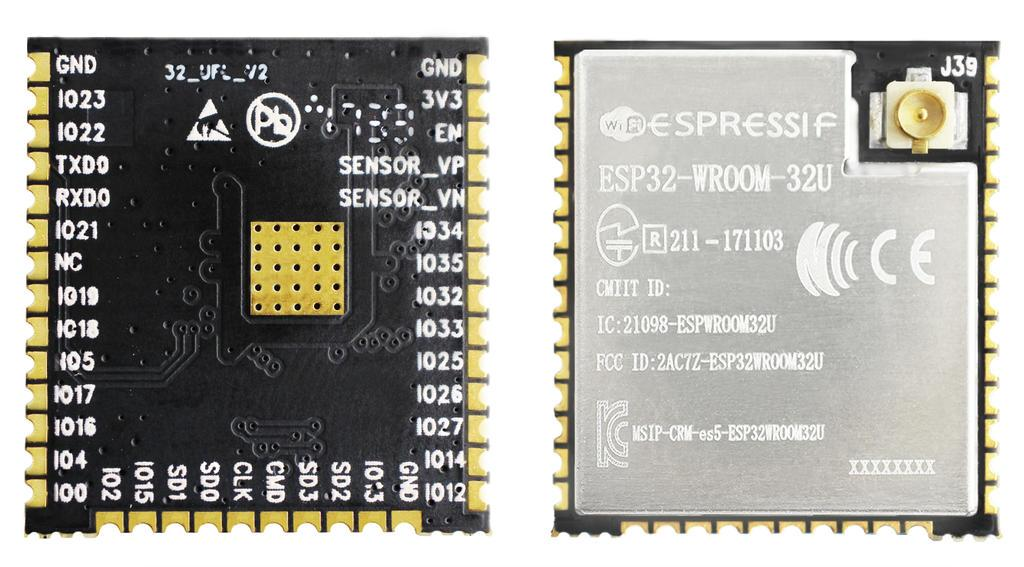
\includegraphics[width = 0.4\textwidth]{graphics/Produktbild_ESP32}
%\caption{ESP32-32U Wroom.}
%\label{fig:Produktbild_ESP32_32U_Wroom}
%\end{figure}
%
%\begin{figure}[!h]
%\center
%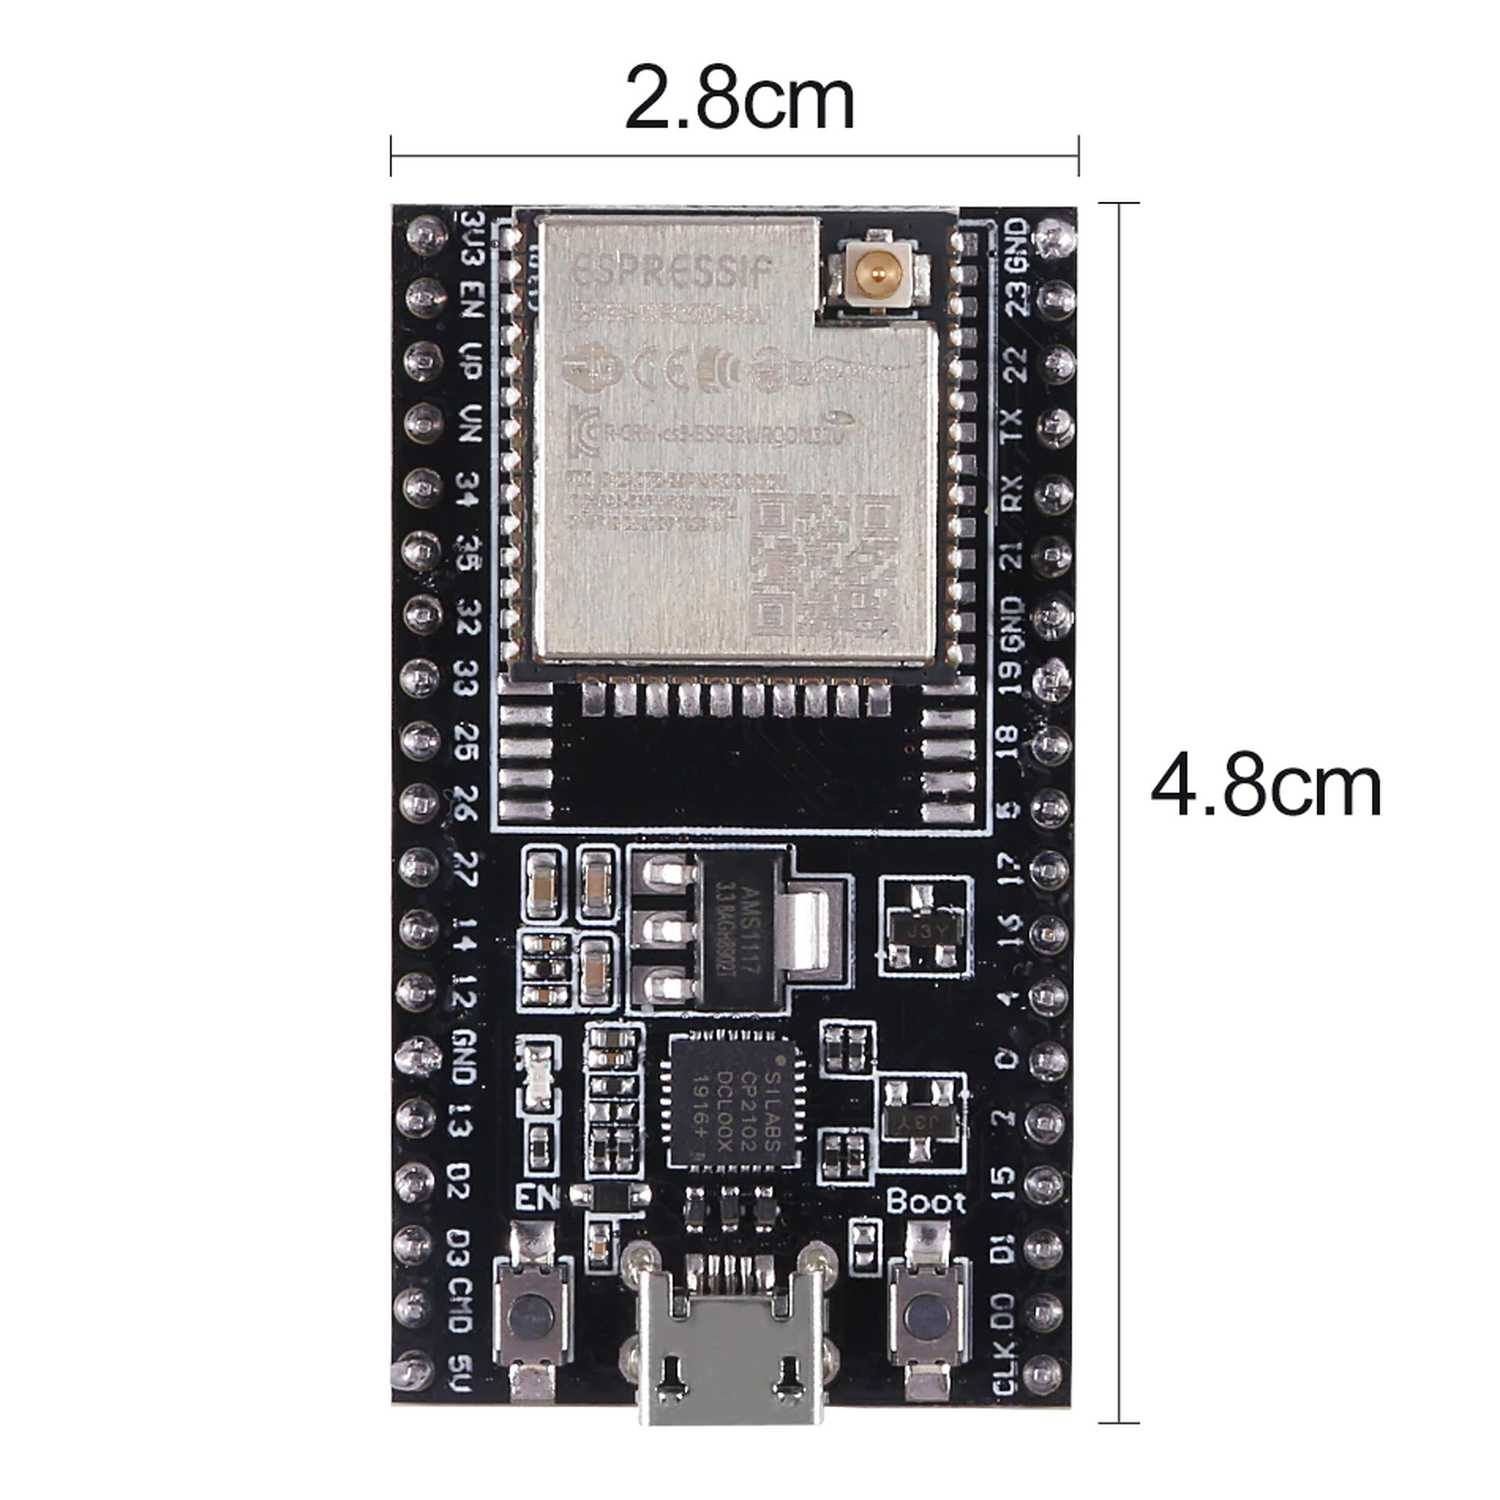
\includegraphics[width = 0.4\textwidth]{graphics/Produktbild_ESP32_2}
%\caption{ESP32-32U DevKit.}
%\label{fig:Produktbild_ESP32_32U_DevKit}
%\end{figure}